\section{Documento dell'architettura software}\label{sec:docarchsoft}
In questa sezione analizzeremo diffusamente il processo di dettagliamento dell'architettura
software, effettuando la distinzione tra lato Amministratore e lato Utente, come
avverrà nelle sottosezioni seguenti. Abbiamo voluto evidenziare il diagramma
degli stati di alcune classi del nostro modello di dominio, tramite la 
Figura \vref{fig:statecharts_domainmodel_one}.

Ci sentiamo di effettuare un'unica precisazione per quanto riguarda la
Figura \vref{fig:statecharts_domainmodel_one}\subref{fig:reservationstate_one}:
con ``modifica del referto'' intendiamo sia la modifica della prenotazione 
dovuta al primo inserimento del documento, sia la modifica effettiva del
referto associato.

Inoltre ci sentiamo di rimarcare l'impossibilità di utilizzare, tramite il
tool \textsc{ArgoUML} i ``combined fragments'': siamo stati conseguentemente
costretti ad apportare le opportune modifiche tramite l'utilizzo di \textsc{Inkscape}.

\begin{figure}[t]
 \centering 
   \subfloat[][\emph{System Message}.]{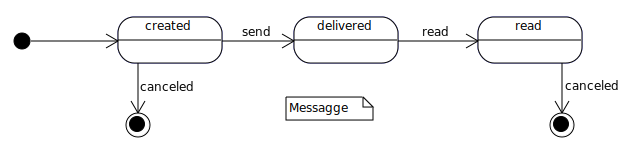
\includegraphics[scale=0.7]{svgs/statechart_messaggio}}\\
   \subfloat[][\emph{Reservation}.]{\label{fig:reservationstate_one}\includegraphics[scale=0.7]{svgs/statechart_prenotazione}}\\
 \caption{\emph{Statecharts for some classes of the Domain Model}.}
 \label{fig:statecharts_domainmodel_one}
\end{figure}

\subsection{Amministratore}
\subsubsection{Vista dei Dati}
\begin{figure}[!t]
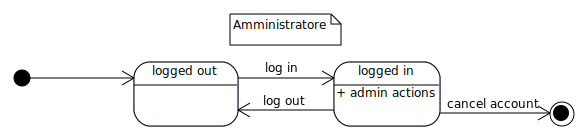
\includegraphics[scale=0.7]{svgs/statechart_amministratore}
\caption{\textit{Administrator's Statechart}.}
\label{fig:statechart_amministratore}
\end{figure}
Possiamo fornire una descrizione dei possibili stati dell'amministratore in
Figura \vref{fig:statechart_amministratore}: nota che, anche se non è prevista
l'eliminazione da interfaccia grafica di un singolo amministratore, questa è
sempre possibile andando ad effettuare modifiche nel database.


\subsubsection{Vista dei Casi d'Uso}
Nella Figura \vref{fig:admin_ucview_one}, mostriamo i primi \textsc{Diagrammi di 
Sequenza} attinenti all'interazione tra Amministratore ed una generica istanza
del Sistema (\texttt{System}). Questi diagrammi fanno riferimento
ai Casi d'Uso descritti nella Sottosezione \vref{subsec:usecasetext}, ed in
particolare ai seguenti:
\begin{itemize}
\diam Contattare l'amministratore (lato Amministratore)
\diam Effettuare una prenotazione (lato Amministratore)
\diam Accedere al sistema (Attore primario: amministratore)
\diam Inserire i referti dei pazienti
\diam Modificare i referti dei pazienti
\diam Gestire le prenotazioni
\end{itemize}

Per ognuna delle operazioni ottenuto dal \textsc{Diagramma di Classe} ``System 
Methods to implement'', definiamo i contratti corrispondenti dettagliati qui
sotto, allo scopo di definire l'interfaccia 
di sistema pubblica dei nostri metodi:
\begin{itemize}
\diam \texttt{getFreeSlotsAfter}
\diam \texttt{fetchReservations}
\diam \texttt{addReport}
\diam \texttt{postponeReservs}
\diam \texttt{Reserve}
\diam \texttt{fetchPendantReq}
\diam \texttt{Login}
\diam \texttt{fetchRemoveReq}
\diam \texttt{fetchPostponeReq}
\diam \texttt{destroyRequestPostpone}
\diam \texttt{freeSlotReserv}
\end{itemize}

Nelle post-condizioni si considerano i suggerimenti forniti all'interno della
Sottosottosezione \vref{subsubsec:aamddomsugg_admin}. \label{subsubsec:adminucaseview}

\begin{figure}[p]
 \centering
   \subfloat[][\emph{Adding Patient's Reservation}.]{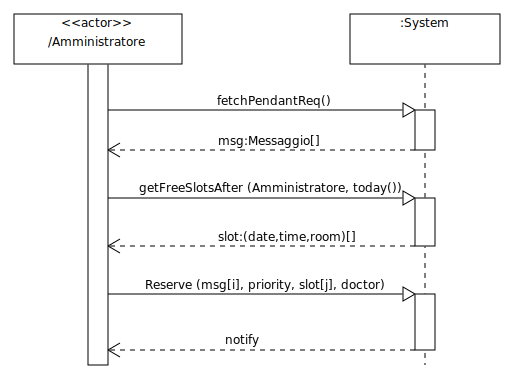
\includegraphics[scale=0.55]{svgs/admin_Prenotazionepaziente}}
   \subfloat[][\emph{Adding Patient's Urgent Reservation}.]{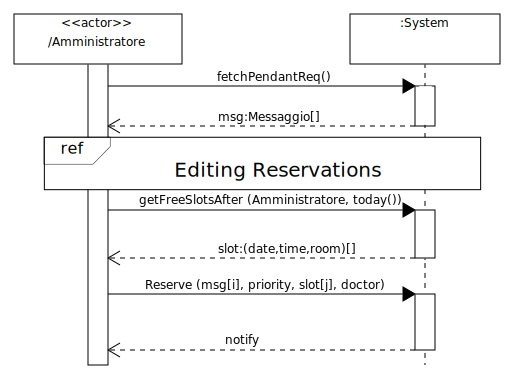
\includegraphics[scale=0.55]{svgs/admin_Prenotazionepaziente_urgente}}\\
   \subfloat[][\emph{Editing Reservations}.]{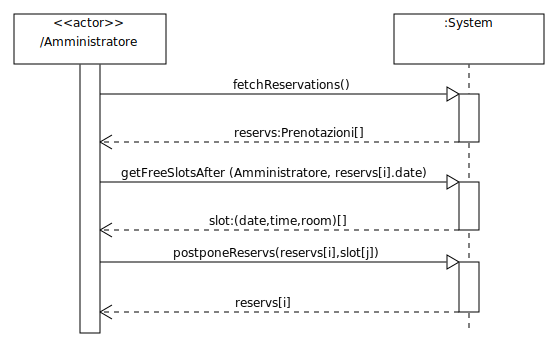
\includegraphics[scale=0.55]{svgs/admin_Modificaprenotazioni}}
   \subfloat[][\emph{Postponing Reservations}.]{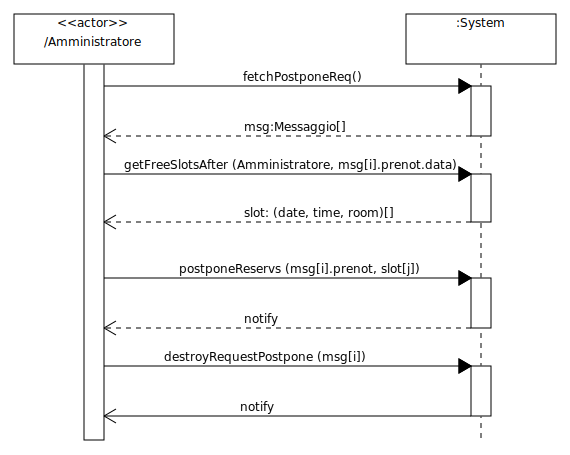
\includegraphics[scale=0.45]{svgs/admin_PosticipaPrenotazione}}\\
   \subfloat[][\emph{Adding Report to Reservations}.]{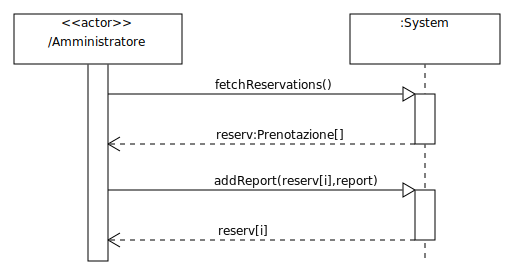
\includegraphics[scale=0.55]{svgs/admin_Inserimentoreferti}}
   \subfloat[][\emph{Authentication}.]{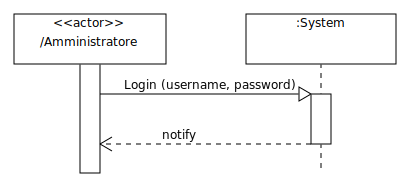
\includegraphics[scale=0.6]{svgs/admin_Accederealsistema}}\\
   \subfloat[][\emph{Editing Reservations' Report}.]{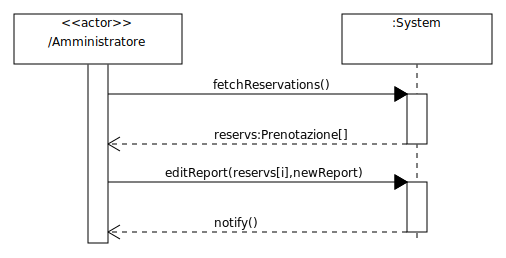
\includegraphics[scale=0.55]{svgs/admin_Modificareferti}}\\
   
 \caption{\emph{Administrator's Use Case View (1)}.}
 \label{fig:admin_ucview_one}
\end{figure}

\begin{figure}[t]
 \centering
   \subfloat[][\emph{Deleting Reservations}.]{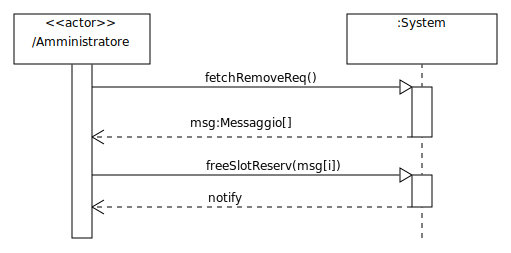
\includegraphics[scale=0.6]{svgs/admin_Cancellazioneprenotazioni}}
   \subfloat[][\hbox{\emph{System Methods to implement}.}]{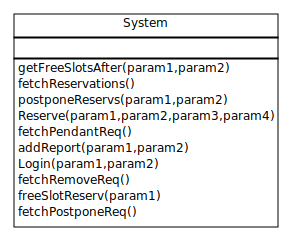
\includegraphics[scale=0.6]{svgs/admin_DiagrammadiClasse}}\\
 \caption{\emph{Administrator's Use Case View (1)}}
\end{figure}

\begin{tabularx}{\columnwidth}{cX}
\toprule
\textsc{Contratto 01}:& \textbf{getFreeSlotsAfter}\\
\midrule
\textit{Operazione}: & 	\texttt{getFreeSlotsAfter(amministratore,time)}\\
\textit{Use Case}: &	Gestire le prenotazioni, Effettuare una prenotazione (lato amministratore)\\
\textit{Pre-condizioni}: &  Nessuna\\
\textit{Post-condizioni}: & \begin{itemize}
\item Sono creati gli \texttt{Slot} $s[]$ non ancora occupati nel sistema a partire
	dal tempo \texttt{time} per il reparto gestito dall'\texttt{amministratore}
	(\textit{creazione di istanza}).
\end{itemize}\\
\bottomrule
\end{tabularx}
\medskip

\begin{tabularx}{\columnwidth}{cX}
\toprule
\textsc{Contratto 02}:& \textbf{fetchReservations}\\
\midrule
\textit{Operazione}: & 	\texttt{fetchReservations()}\\
\textit{Use Case}: &	Inserire i referti dei pazienti, Modificare i referti 
			dei pazienti, Gestire le prenotazioni\\
\textit{Pre-condizioni}: &  Sono presenti delle prenotazioni all'interno del
			sistema che devono essere gestite\\
\textit{Post-condizioni}: & \begin{itemize}
\item Sono ottenute le \texttt{Prenotazioni} $p[]$ memorizzate all'interno del sistema,
	ed associate all'\texttt{Amministratore} $admin.reservations = p[]$
	(\textit{creazione di istanza}).
\end{itemize}\\
\bottomrule
\end{tabularx}
\medskip


\begin{tabularx}{\columnwidth}{cX}
\toprule
\textsc{Contratto 03}: & 	\textbf{addReport}\\
\midrule
\textit{Operazione}: & 	\texttt{addReport(prenotazione,report)}\\
\textit{Use Case}: &	Inserire i referti dei pazienti\\
\textit{Pre-condizioni}: &  L'amministratore associa un Referto alla Prenotazione
			a cui ha fatto seguito la vista che l'ha generato.\\
\textit{Post-condizioni}: & \begin{itemize}
\item È associata la prenotazione $prenotazione$ ad un Referto esistente: $prenotazione.referto = report$
(\textit{associazione formata}).
\end{itemize}\\
\bottomrule
\end{tabularx}
\medskip

\begin{tabularx}{\columnwidth}{cX}
\toprule
\textsc{Contratto 04}:& \textbf{postponeReservs}\\
\midrule
\textit{Operazione}: & 	\texttt{postponeReservs(prenotazione,newSlot)}\\
\textit{Use Case}: &	Contattare l'amministratore (lato Amministratore), Gestire le prenotazioni\\
\textit{Pre-condizioni}: &  Mentre per quanto concerne \textit{Contattare l'amministratore}
			è necessario che un utente abbia effettuato la richiesta,
			nel secondo caso è necessario che sia pervenuta una
			richiesta da un utente.\\
\textit{Post-condizioni}: & \begin{itemize}
\item È liberato lo Slot temporale $prenotazione.slot$ associato alla Prenotazione (\textit{cancellazione
	di istanza})
\item All'interno della Prenotazione, l'associazione dello Slot liberato 
	precedentemente è sostituita  con un nuovo Slot temporale ottenuto tra 
	quelli disponibili $newSlot$ (\textit{associazione formata})
\item È creata una nuova istanza $msg$ di \textit{MAmministratore} (\textit{creazione di istanza})
\item È settataa la tipologia $msg.kind$ del messaggio a $defer$ (\textit{modifica di attributo})
\item È associato il mittente nel messaggio dalla \texttt{Prenotazione}: $msg.mittente = 
	newSlot.sala.amministratore$ (\textit{associazione formata})
\item È associato il destinatario nel messaggio dalla \texttt{Prenotazione}: $msg.destinatario 
	= prenotazione.paziente$ (\textit{associazione formata})
\item È associata la prenotazione al messaggio: $msg.prenotazione = prenotazione$
	(\textit{associazione formata})
\end{itemize}\\
\bottomrule
\end{tabularx}
\medskip




\begin{tabularx}{\columnwidth}{cX}
\toprule
\textsc{Contratto 05}:& \textbf{Reserve}\\
\midrule
\textit{Operazione}: & 	\texttt{Reserve(messaggio,valPriorità,newSlot,dottore)}\\
\textit{Use Case}: &	Effettuare una prenotazione (lato Amministratore)\\
\textit{Pre-condizioni}: &  Un utente richiede di effettuare una visita tramite 
			l'invio di un \texttt{Messaggio} all'amministratore.\\
\textit{Post-condizioni}: & \begin{itemize}
\item È stata creata una nuova Prenotazione $p$ (\textit{creazione di istanza})
\item È stata associata alla Prenotazione il Paziente, contenuto all'interno del 
	messaggio: $p.paziente = messaggio.mittente$ (\textit{associazione formata}).
\item È stata associata alla Prenotazione uno Slot temporale tra quelli disponibili:
	$p.slot = newSlot$ (\textit{associazione formata}).
\item È stata associata alla Prenotazione una Priorità di visita: $p.priorita = Priorità$ (\textit{modifica di attributo})
\item È stata associata alla Prenotazione un Medico curante: $p.dottore = dottore$ (\textit{modifica di attributo})
\item È creata una nuova istanza $msg$ di \textit{MAmministratore} (\textit{creazione di istanza})
\item È settata la tipologia $msg.kind$ del messaggio a $reserve$ (\textit{modifica di attributo})
\item È associato il mittente del messaggio: $msg.mittente = 
	messaggio.destinatario$ (\textit{associazione formata})
\item È associato il destinatario del messaggio: $msg.destinatario 
	= msg.mittente$ (\textit{associazione formata})
\item È associata la prenotazione al messaggio: $msg.prenotazione = p$
	(\textit{associazione formata})
\item È rimossa l'istanza di $messaggio$ (\textit{cancellazione di istanza}). 
\end{itemize}\\
\bottomrule
\end{tabularx}
\medskip



\begin{tabularx}{\columnwidth}{cX}
\toprule
\textsc{Contratto 06}:& \textbf{fetchPendantReq}\\
\midrule
\textit{Operazione}: & 	\texttt{fetchPendantReq()}\\
\textit{Use Case}: &	Effettuare una prenotazione (lato Amministratore)\\
\textit{Pre-condizioni}: &  Nessuna\\
\textit{Post-condizioni}: & \begin{itemize}
\item Sono associate le nuove istanze dei messaggi $msgs[]$ di richiesta di visita 
	all'\texttt{Amministratore} compentente in $admin.messages$ (\textit{modifica di attributo})
\end{itemize}\\
\bottomrule
\end{tabularx}
\medskip


\begin{tabularx}{\columnwidth}{cX}
\toprule
\textsc{Contratto 07}: & 	\textbf{Login}\\
\midrule
\textit{Operazione}: & 		\texttt{Login(Username,Password)}\\
\textit{Riferimento (Use Case)}: &	Accedere al sistema (Attore primario: amministratore)\\
\textit{Pre-condizioni}: &  	Nessuna\\
\textit{Post-condizioni}: & 	\begin{itemize}
\item È stata creata un'istanza $g$ della classe \texttt{Guest}.
\item Si setta l'attributo $g.kind$ o $isOrthopedic$ o $isPediatrics$ affermativamente nel 
	caso in cui l'amministratore afferisca al reparto di ortopedia o a quello di pediatria.
\item È settato l'attributo $g.logged$ a $true$ se l'autenticazione è avvenuta
	con successo.
\end{itemize}\\
\bottomrule
\end{tabularx}
\medskip

\begin{tabularx}{\columnwidth}{cX}
\toprule
\textsc{Contratto 08}: & 	\textbf{fetchRemoveReq}\\
\midrule
\textit{Operazione}: & 		\texttt{fetchRemoveReq()}\\
\textit{Riferimento (Use Case)}: &	Contattare l'amministratore (lato Amministratore)\\
\textit{Pre-condizioni}: &  	Almeno un utente invia all'amministratore la
				richiesta di cancellazione della visita.\\
\textit{Post-condizioni}: & 	\begin{itemize}
\item I nuovi messaggi di cancellazione $msgsdel[]$ della visita sono associati all'amministratore
	compentente: $admin.messagesdel = msgsdel[]$ (\textit{modifica di attributo})
\end{itemize}\\
\bottomrule
\end{tabularx}
\medskip


\begin{tabularx}{\columnwidth}{cX}
\toprule
\textsc{Contratto 09}: & 	\textbf{fetchPostponeReq}\\
\midrule
\textit{Operazione}: & 		\texttt{fetchPostponeReq()}\\
\textit{Riferimento (Use Case)}: &	Contattare l'amministratore (lato Amministratore)\\
\textit{Pre-condizioni}: &  	Almeno un utente invia all'amministratore la
				richiesta di posticipazione della visita.\\
\textit{Post-condizioni}: & 	\begin{itemize}
\item I nuovi messaggi di richiesta di posticipazione $msgspost[]$ della visita sono associati all'amministratore
	compentente: $admin.messagespost = msgspost[]$ (\textit{modifica di attributo})
\end{itemize}\\
\bottomrule
\end{tabularx}
\medskip

\begin{tabularx}{\columnwidth}{cX}
\toprule
\textsc{Contratto 10}: & 	\textbf{destroyRequestPostpone}\\
\midrule
\textit{Operazione}: & 		\texttt{destroyRequestPostpone(msg)}\\
\textit{Riferimento (Use Case)}: &	Contattare l'amministratore (lato Amministratore),
				Gestire le prenotazioni.\\
\textit{Pre-condizioni}: &  	L'amministratore deve aver gestito la richiesta di
				spostamento contenuta nel messaggio.\\
\textit{Post-condizioni}: & 	\begin{itemize}
\item È cancellata l'istanza $msg$ (\textit{cancellazione})
\end{itemize}\\
\bottomrule
\end{tabularx}
\medskip


\begin{tabularx}{\columnwidth}{cX}
\toprule
\textsc{Contratto 11}: & 	\textbf{freeSlotReserv}\\
\midrule
\textit{Operazione}: & 		\texttt{freeSlotReserv(messaggio)}\\
\textit{Riferimento (Use Case)}: &	Contattare l'amministratore (lato Amministratore)\\
\textit{Pre-condizioni}: &  	Almeno un utente invia all'amministratore la
				richiesta di cancellazione della visita.\\
\textit{Post-condizioni}: & 	\begin{itemize}
\item È creata una nuova istanza $msg$ di \textit{MAmministratore} (\textit{creazione di istanza})
\item È settata la tipologia $msg.kind$ del messaggio a $revoke$ (\textit{modifica di attributo})
\item È associato il mittente del messaggio: $msg.mittente = 
	messaggio.destinatario$ (\textit{associazione formata})
\item È associato il destinatario del messaggio: $msg.destinatario 
	= msg.mittente$ (\textit{associazione formata})
\item È associato il contenuto testuale al messaggio: $msg.content = p.toText()$
	(\textit{associazione formata})
\item È eliminata una istanza di Prenotazione $\pi$ precedentemente inviata dal 
	Paziente $p$, che è indicata all'interno del messaggio nell'attributo
	$message.prenotazione$ (\textit{cancellazione di istanza}).
\item È rimossa l'istanza di $messaggio$ (\textit{cancellazione di istanza}). 
\end{itemize}\\
\bottomrule
\end{tabularx}
\medskip




